\documentclass[a4paper,11pt]{article}
\usepackage[left=2cm,right=2cm,
top=2cm,bottom=2cm,bindingoffset=0cm]{geometry}

%%% Работа с русским языком
\usepackage{cmap}					% поиск в PDF
\usepackage{mathtext} 				% русские буквы в формулах
       			% Использование кода в файле
\usepackage[T2A]{fontenc}			% кодировка
\usepackage[utf8]{inputenc}			% кодировка исходного текста
\usepackage[english,russian]{babel}	% локализация и переносы
     % Enables syntax highlighting for code listings.
%%% Дополнительная работа с математикой

\usepackage{amsmath,amsfonts,amssymb,amsthm,mathtools} % AMS
\usepackage{icomma} % "Умная" запятая: $0,2$ --- число, $0, 2$ --- перечисление
%% Номера формул
\mathtoolsset{showonlyrefs=false} % Показывать номера только у тех формул, на которые есть \eqref{} в тексте.
%\usepackage{leqno} % Нумерация формул слева

%% Свои команды
%\DeclareMathOperator{\sgn}{\mathop{sgn}}

%% Перенос знаков в формулах (по Львовскому)
%\newcommand*{\hm}[1]{#1\nobreak\discretionary{}
	%	{\hbox{$\mathsurround=0pt #1$}}{}}

%%% Работа с картинками
\usepackage{graphicx}  % Для вставки рисунков
\graphicspath{{images/}{images2/}}  % папки с картинками
\setlength\fboxsep{3pt} % Отступ рамки \fbox{} от рисунка
\setlength\fboxrule{1pt} % Толщина линий рамки \fbox{}
\usepackage{wrapfig} % Обтекание рисунков текстом

%%% Работа с таблицами
\usepackage{array,tabularx,tabulary,booktabs} % Дополнительная работа с таблицами
\usepackage{longtable}  % Длинные таблицы
\usepackage{multirow} % Слияние строк в таблице

%%% Теоремы
%\theoremstyle{plain} % Это стиль по умолчанию, его можно не переопределять.
%\newtheorem{theorem}{Теорема}[section]
%\newtheorem{proposition}[theorem]{Утверждение}

%\theoremstyle{definition} % "Определение"
%\newtheorem{corollary}{Следствие}[theorem]
%\newtheorem{problem}{Задача}[section]

%\theoremstyle{remark} % "Примечание"
%\newtheorem*{nonum}{Решение}

%%% Программирование
%\usepackage{etoolbox} % логические операторы

%%% Страница
%\usepackage{extsizes} % Возможность сделать 14-й шрифт
%\usepackage{geometry} % Простой способ задавать поля
%\geometry{top=25mm}
%\geometry{bottom=35mm}
%\geometry{left=35mm}
%\geometry{right=20mm}
%
%\usepackage{fancyhdr} % Колонтитулы
% 	\pagestyle{fancy}
%\renewcommand{\headrulewidth}{0pt}  % Толщина линейки, отчеркивающей верхний колонтитул
% 	\lfoot{Нижний левый}
% 	\rfoot{Нижний правый}
% 	\rhead{Верхний правый}
% 	\chead{Верхний в центре}
% 	\lhead{Верхний левый}
%	\cfoot{Нижний в центре} % По умолчанию здесь номер страницы

\usepackage{setspace} % Интерлиньяж
%\onehalfspacing % Интерлиньяж 1.5
%\doublespacing % Интерлиньяж 2
%\singlespacing % Интерлиньяж 1

\usepackage{lastpage} % Узнать, сколько всего страниц в документе.

\usepackage{soul} % Модификаторы начертания

\usepackage{hyperref}
\usepackage[usenames,dvipsnames,svgnames,table,rgb]{xcolor}
\hypersetup{				% Гиперссылки
	unicode=true,           % русские буквы в раздела PDF
	pdftitle={Заголовок},   % Заголовок
	pdfauthor={Автор},      % Автор
	pdfsubject={Тема},      % Тема
	pdfcreator={Создатель}, % Создатель
	pdfproducer={Производитель}, % Производитель
	pdfkeywords={keyword1} {key2} {key3}, % Ключевые слова
	colorlinks=true,       	% false: ссылки в рамках; true: цветные ссылки
	linkcolor=red,          % внутренние ссылки
	citecolor=black,        % на библиографию
	filecolor=magenta,      % на файлы
	urlcolor=cyan           % на URL
}

\usepackage{csquotes} % Еще инструменты для ссылок

%\usepackage[style=authoryear,maxcitenames=2,backend=biber,sorting=nty]{biblatex}

\usepackage{multicol} % Несколько колонок

%\usepackage{tikz} % Работа с графикой
%\usepackage{pgfplots}
%\usepackage{pgfplotstable}

\usepackage{titlesec}
\usepackage[most]{tcolorbox} % для управления цветом

\definecolor{block-gray}{gray}{1.00} % уровень прозрачности (1 - максимум)
\newtcolorbox{myquote}{colback=block-gray,grow to right by=-4mm,grow to left by=-4mm,
	boxrule=1pt,boxsep=0pt,breakable} % настройки области с изменённым фоном

\renewcommand{\phi}{\ensuremath{\varphi}}
\renewcommand{\epsilon}{\ensuremath{\varepsilon}}
\renewcommand{\kappa}{\ensuremath{\varkappa}}
\author{Злагода А. В.}
\title{Приминение генерации плазмы в ионных двигателях}




\begin{document}
\begin{center}
\center{ \bf Государственное Бюджетное Учреждение дополнительного образования «Ленинградский областной центр развития творчества одаренных детей и юношества «Интеллект»}
\end{center}
\noindent\makebox[\linewidth]{\rule{\textwidth}{2pt}}
\begin{center}
	\Huge \bf Приминение генерации плазмы в ионных двигателях 
\end{center}

\hfill\Large
\vbox{%
\hfill%
\vbox{%
\hbox{\textbf{Автор:}}%
\hbox{Злагода Алексей}%
%\hbox{\textbf{Руководители:}}%
%%\hbox{Макаренко А. О.}%
%\hbox{Чугунов С. С}%
}%
} 

\section{\Large  Введение}

\indent
В эпоху освоения космоса появляется необходимость в дальних путешествиях, что затрачивают огромное количество ресурсов.
Из формулы Циолковского 
$v_\text{кор} = v_\text{топл} \ln(\frac{M_\text{нач}}{M_\text{кон}})$ 
следует, что скоростей, необходимых для покидания пределов земли 
$(11.2\frac{\text{км}}{\text{с}})$
 и пределов солнечной системы 
 $(16.7\frac{\text{км}}{\text{с}})$
 необходимо либо использовать крайне большие потери в массе, либо использовать большие скорости топлива, либо комбинировать эти два параметра для достижения оптимальных режимов.   
При этом необходимо учитывать, что существуют ограничения в габаритах космических аппаратов, и, соответсвенно, ограничение по запасу топлива. Поэтому необходимо увеличивать скорость вылета топлива. 
\newline
\indent
В современных двигателях скорость вылета рабочего тела приблизительно равна 5 км/c, что достаточно далеко от максимально возможной скорости движения объектов во вселенной. В связи с чем можно оптимизировать расход топлива, приблизив скорость вылета объектов к световой.
\section{\Large Актуальность}
Как было сказано ранее, увеличение скорости вылета рабочего тела позволит увеличить экономичность ракет, и, как следствие, удешевить каждый старт. 
\newpage
\begin{figure}[h!]
	\centering
	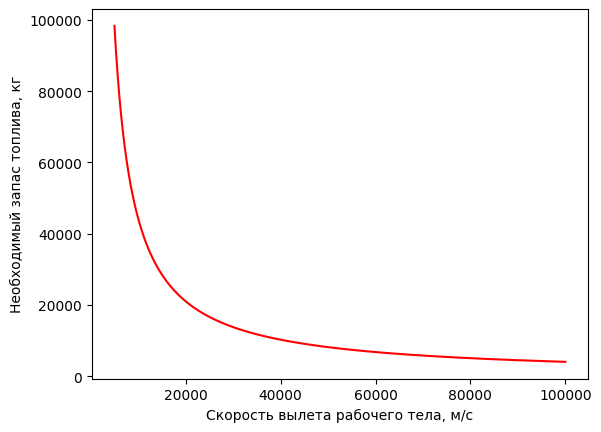
\includegraphics[width=0.5\textwidth]{"media/M_fuel_by_WTS.png"}
	\caption{График Зависимость необходимого запаса топлива от скорости вылета рабочего тела при изменении скорости на 2 км/с и "сухой" массе корабля, равной 200т}
\end{figure}


На графике представлена зависимость необходимого запаса топлива от скорости вылета рабочего тела. 
Очевидно, что при увеличении скорости даже на два порядка получается весьма значительный выигрыш в топливе.
\newline
\indent
Вторая проблема, заключается в невозможности реализовать этот выигрыш с помощью химических двигателей. 
Поэтому возникает необходимость в исследовании новых схем ускорения рабочего тела.





\section{\Large Существующие схемы}

Полсе обзора литературы было выяснено, что существуют схемы, пригодные к использованию в космическом пространстве. Таковыми являются: 
\begin{enumerate}
	\item Ионные двигатели
	\item Стационарные плазменные двигатели [4]
\end{enumerate}
\subsection{Ионные двигатели}
Ионный двигатель — тип электрического ракетного двигателя, принцип работы которого основан на создании реактивной тяги на базе ионизированного газа, разогнанного до высоких скоростей в электрическом поле. 
\newline
Ионный двигатель характеризуется малой тягой и высоким удельным импульсом. Ресурс работы оценивается в диапазоне 10 тысяч — 100 тысяч часов. В настоящее время разрабатывается новое поколение ионных двигателей, рассчитанных на расход 450 килограммов ксенона, чего хватит на 22 тысячи часов работы при максимальном форсаже. Причинами отказа могут стать износ ионной оптики, катодной диафрагмы и держателя для плазмы, истощение рабочего материала в каждой катодной вставке и откол материала в разрядной камере. Согласно проведённым тестам при удельном импульсе больше 2000 с первым произойдёт структурный отказ ионной оптики при использовании 750 килограммов топлива, что в 1,7 раза превышает квалификационные требования. При удельном импульсе меньше 2000 с прототип может удвоить расход потребляемого топлива

\subsection{Стационарные плазменные двигатели}
Стационарный плазменный двигатель (СПД) — это одна из разновидностей электроракетного двигателя, где электрическая энергия используется для ионизации газа и придания полученной плазме высокой скорости истечения из «сопла». 
У такого двигателя нет топлива в привычном понимании, т.е. горючего и окислителя, 
необходимого для химической реакции с выделением тепла. СПД подходит практически любой газ, но лучше использовать химически неактивные и с высокой атомной массой, вроде аргона или ксенона. Плазменные двигатели обеспечивают очень высокую скорость выбрасываемой струи газа, например, для ксенона это около 30 км/с. Для сравнения, скорость выброса газа у одного из самых эффективных химических ракетных двигателей — кислород-водородного — около 4,5 км/с. Преимуществом химических двигателей является способность выбрасывать сразу много газа, что дает большую тягу. СПД же требует мощного источника электрической энергии, и даже с ним способен выбрасывать лишь незначительную массу газа за момент времени, то есть имеет очень малую тягу и требует много времени на разгон и торможение. Плазменные двигатели применяются только в космосе: оснащенные ими космические аппараты имеют относительно малый запас рабочего тела и большой размах солнечных батарей.
\section{\Large Постановка задачи}
Существует гипотеза, что возможно создать достаточно большую тягу, комбинируя два вышеописанных подхода. 
В частноси предлагается использовать термоядерную реакцию для разложения вещества, предположительно, дейтерия, на ионы и электроны. 
После предполагается перемещать ионы в электрическое поле, в котором они будут ускоряться до больших скоростей и в дальнейшем покидать корабль, предавая ему ускорение.
Термоядерная реакция будет обеспечивать высокую степень ионизации[3], а электрическое поле - увеличение скорости движения ионов. 

\newpage
\section{Используемая Литература и веб ресурсы}
\begin{enumerate}
	\item Исследование режимов термоядерного горения. Светлов А.С. УДК 621.039.6
	\item МОДЕЛИРОВАНИЕ ТЕРМОЯДЕРНОЙ УСТАНОВКИ С ВНУТРЕННИМ КАТАЛИТИЧЕСКИМ ЦИКЛОМ С.Н. Столбов, Ю.В. Дробышевский, И.М. Анфимов, В.А. Варлачев, С.П. Кобелева, С.А. Некрасов, Корженевский А.В. DOI 10.26583/npe.2021.2.13
	\item Основы физики плазмы (2-е изд., испр. и доп.) Голант В. Е., Жилинский А. П., Сахаров И. Е. pp. 448 (2011) Links: LibSTC.cc WorldCat: isbn:5811411987 	ISBN: 5811411987, 9785811411986  Publisher: Издательство "Лань" 
	\item https://habr.com/ru/articles/448088/
\end{enumerate}


%\noindent 
%\subsection{Графики}
%\noindent
%\subsection{Таблицы}
%\noindent
%Полезные шаблоны
%Случайная погрешность

%\[
%\sigma = \sum\limits_{i = 1}^n (\sqrt{\dfrac{(x_i - \langle x \rangle)^2}{N(N-1)}})
%\]

%Метод наименьших квадратов
%
%Для нахождения коэффициентов A, C зависимости $Y(X) = AX + C$
%\begin{multicols}{2}
%
%\begin{equation}
%	\overline{X} = \dfrac{1}{N} \sum\limits_{i = 1}^N X_i
%\end{equation}
%
%\begin{equation}
%	D = \sum\limits_{i = 1}^N (X_i - \overline{X})^2
%\end{equation}
%
%\begin{equation}
%	A = \dfrac{1}{D} \sum\limits_{i = 1}^N (X_i - \overline{X})Y_i
%\end{equation}
%
%\begin{equation}
%	\Delta A = \sqrt{\dfrac{E}{D}}
%\end{equation}
%
%\begin{equation}
%	\overline{Y} = \dfrac{1}{N} \sum\limits_{i = 1}^N Y_i
%\end{equation}
%
%\begin{equation}
%	E = \dfrac{1}{N-2} \sum\limits_{i = 1}^N(Y_i - AX_i - C)^2	
%\end{equation}
%
%\begin{equation}
%	C = \overline{Y} - A \overline{X}
%\end{equation}
%
%\begin{equation}
%	\Delta C = \sqrt{\left(\dfrac{1}{N} + \dfrac{\overline{X}^2}{D} \right) \cdot E}
%\end{equation}
%
%\end{multicols}

\end{document}